High-dimensionality forms an obstacle to the analysis of many complex systems.
That is widely agreed, even though the degree as to which it applies is strongly dependent on the academic field.
The so-called \emph{curse of dimensionality} \cite{Optim:Bellman1957,Optim:Bellman1961} very generally
refers to difficulties in the characterization of high-dimensional objects with discrete information.
Various different manifestations of this problem are related to the volume and geometry of high-dimensional spaces.
They play a major role in much of machine learning \cite{ML:Bishop2006,ML:Murphy2012}, learning theory \cite{Statistics:Kulkarni2011,Statistics:James2013}
and multivariate statistics \cite{Statistics:Izenman2008,Statistics:Koch2014}.
\par % SOME EXAMPLES
Examples that are often used to illustrate the immense volume and the counterintuitive behavior of Euclidean norms and distances in high-dimensional spaces include the following.
The volume of a hypersphere with fixed radius, e.g.\ a unit hypersphere embedded into a unit hypercube whose volume is always one, drops to zero.
Most of the volume of a high-dimensional sphere is located in a thin shell underneath its surface, rather than in the interior.
Similarly, most of the probability mass of a multivariate Gaussian distribution concentrates around a shell distant from the expected value, rather than in the bell.
% UNIFORM GRID
In one, two and three space dimensions, data points on a regular grid occupying a unit interval, square and cube are shown in \cref{fig:UQ:CurseOfDimensionality}, respectively.
In order to ensure a consistent coverage of the space, the sample size has to grow exponentially with the dimensionality.
Vice versa, uniform data with a fixed sample size quickly become isolated.
% FIGURE: CURSE OF DIMENSIONALITY
\begin{figure}[htbp]
  \centering
  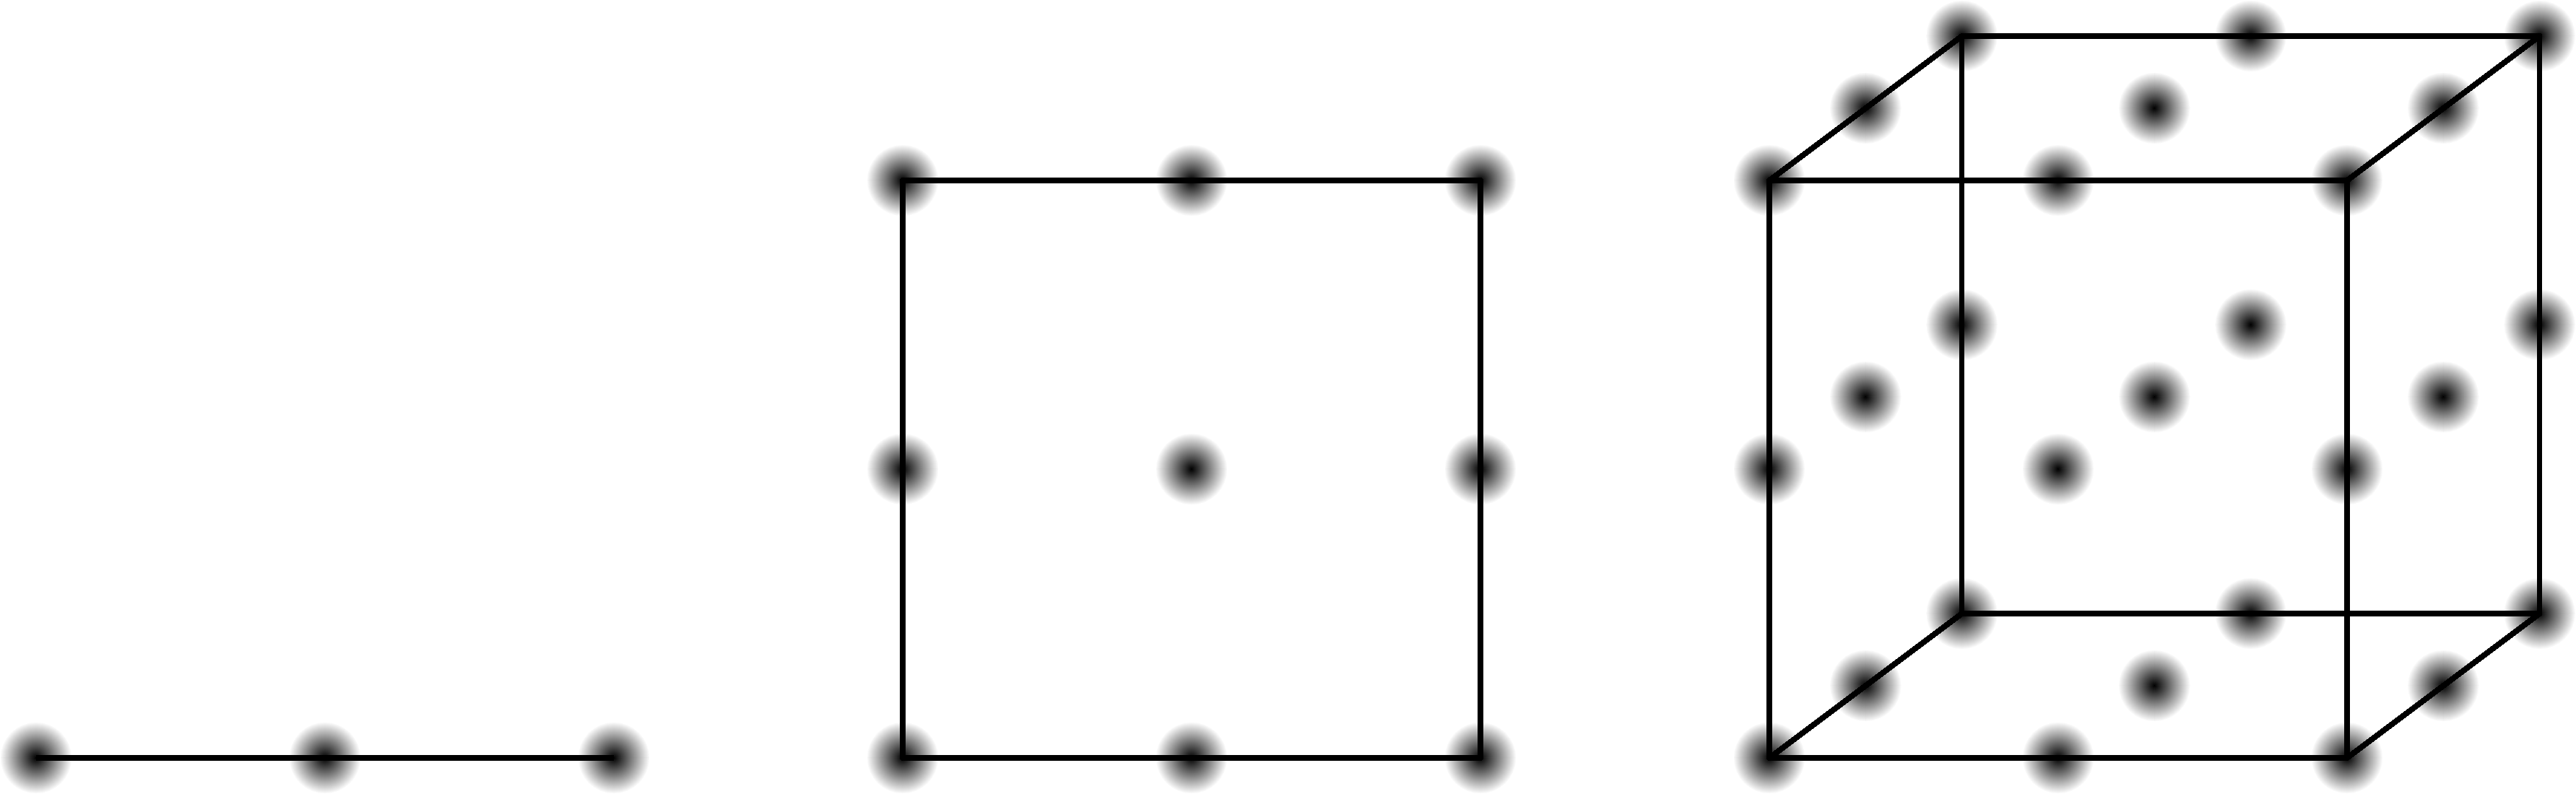
\includegraphics[width=9cm]{fig_UQ_CurseOfDimensionality}
  \caption[Curse of dimensionality]{Curse of dimensionality.}
  \label{fig:UQ:CurseOfDimensionality}
\end{figure}
\par % EXPERIMENTAL DESIGN
The empty space phenomenon immediately shows up in UQ problems for the experimental design in \cref{eq:PCE:ExperimentalDesign}.
Training sets with a fixed sample size fail to representatively cover the input space.
A sufficient coverage would require an exploding number of training runs and is therefore computationally infeasible.
% HIGH-DIMENSIONAL FUNCTION
The curse of dimensionality manifests also in \cref{eq:PCE:Cardinality} which obstructs the expansion of high-dimensional functions in terms of high-order polynomials.
Yet another instantiation of the problem is in \cref{eq:UQ:VectorModel} where all high-dimensional model outputs must be considered individually.
\par % BREAKING THE CURSE
Confronted with this seemingly hopeless situation, one may contemplate surrender.
But fortunately there is the blessing of \emph{sparsity},
i.e.\ real-world problems in high-dimensional ambient spaces often feature characteristic low-dimensional sub-structures that are hidden at the first sight.
By uncovering such essential patterns of information one can break or at least try to smother the curse.
% INPUT DIMENSIONALITY
Given a real data set with many features, techniques for data dimensionality reduction can be applied \cite{Statistics:Lee2007}.
Given an engineering model, a subset of important directions in the multi-dimensional input space can be identified \cite{Uncertainty:Constantine2014}.
% COMPRESSIVE SENSING
Another type of sparsity can be sought after directly in the representation of a signal \cite{Statistics:Foucart2013}.
A hypothetical basis that already contains the actual signal would precisely require that one term.
Even though this case is improbable, sparse recovery methods can be applied in contexts where a favorable basis is known.
\par % THESIS CONNECTION
The solution of complex engineering problems in the UQ domain often requires to use a combination of methods for tackling high-dimensionality at the various modeling levels.
An example can be found in \cref{sec:Hydrology} wherein a hydrological simulator with a collapsed input space will be analyzed.
Also the dimension of the simulator response will be reduced.
After that a regularized least squares problem will be solved that seeks sparsity in the functional basis expansion.